%\addbibresource{/home/jorgsk/Dropbox/phdproject/bibtex/jorgsk.bib}
\subsection{Model of initial transcription}
A highly descriptive kinetic model of initial transcription is required to fit
rate constants with confidence. Several previuosly published kinetic models of
transcription are based on Michaelis Menten kinetics, where the translocation
step is assumed at equilibrium and calculated from free energy parameters of
the RNA-DNA hybrid and the DNA bubble, and where
the Michaelis Menten parameters are estimated from model fitting
\cite{guajardo_model_1997, bai_sequence-dependent_2004,
bai_mechanochemical_2007, tadigotla_thermodynamic_2006}. Here, we use a
different approach. Our model is based on a minimal descriptive scheme for
initial transcription, containing only reactions for i) the forward nucleotide
addition cycle (NAC), ii) backstepping (the first backtracking step), iii)
promoter escape, and iv) backtracking and abortive RNA release (Figure
\ref{fig:model_and_rates}A). The model contains three tunable parameters:
the rate constants for the NAC, the abortive step, and for backtracking and
abortive RNA release (the latter referred to in combination as the abortive
step). We obtain the rate constant for backstepping indirectly from the rate
constant of the NAC. To do so, we make use of pre-calculated abortive
probabilities\cite{hsu_quantitative_1996} (APs), which are available for the
N25 promoter and several ITS variants of this promoter
\cite{hsu_initial_2006}. By making the assumption that the APs reflect
probabilities of backstepping, we can use the fact that this step is in
kinetic competition with the NAC to calculate the rate constant of
backstepping at each position:

\begin{equation*}
  b = \frac{\text{NAC}\cdot \text{AP}}{1-\text{AP}},
\end{equation*}

Figure~\ref{fig:model_and_rates}B shows the initial transcription kinetic scheme
together with placeholder values for the estimated rate constants.
The rate of FL product synthesis upon promoter escape is given by NAC/d
where d is the number of nucleotides from promoter escape until runoff.

In this work we consider APs calculated from initial transcription both in the
presence of GreB (+GreB) and in the absence of GreB (-GreB). When GreB is
present, backtracked complexes may be rescued by GreB stimulated cleavage of
the unaligned 3\ppp end of the transcript. Therefore, APs obtained in the
presence of GreB represent the probability to both backstep and to avoid
resuce by GreB until abortive RNA release. Here, we assume that GreB-mediated
cleavage is rapid compared to the NAC and to backtracking. Since the NAC has
been found to not be rate limiting for the kinetics of initial transcription,
we assume that the repeated NACs before promoter escape caused by
GreB-mediated rescue do reduce the ability of the model to fit +GreB data.

\subsection{Implementation and parameter estimation}
To solve the kinetic scheme we use the direct method for the stochastic
simulation algorithm \cite{gillespie_exact_1977} as implemented in the StocPY
software \cite{maarleveld_stochpy:_2013}. By using stochastic simulations, we
are able to simulate transcription to the level of single RNA polymerases to
resolve some of the stochasticity inherent with such low copy number
reactions. The data we fit our model to is the distribution of time spent in
abortive cycling prior to promoter escape as reported by Revyakin et.\ al
\cite{revyakin_abortive_2006}. This experiment was performed using 100
single-RNAP transcription events (Figure 4D in Revyakin et.\ al), which
motivated our use of stochastic simulations.

We estimate the rate constants of NAC, promoter escape, and unscrunching using an
iterative heuristic process. In the first iteration, we sample uniformly 1000
times values for the three rate constants in the range 1 s$^{-1}$ to 25
s$^{-1}$, which we considered to be reasonable boundaries for rate constants
of all three reactions. For each sample, we use the value for NAC to obtain
rate constants for backstepping (as illustrated in
Figure~\ref{fig:model_and_rates}B). We then use the sampled and calculated
rate constants to simulate initial transcription on N25 with 100 RNAPs and
find the cumulative distribution of time spent in abortive cycling, which is
compared to the measured values from Revaykin et.\ al
\cite{revyakin_abortive_2006} using the root mean squared distance metric.
After all 1000 simulations are finished, we rank them by the metric distance (lower is
better) and calculate the weighted mean and weighted standard deviation of the
top 20 samples, using the inverse of the metric distance as weights, normalized
so the closest fit has weight 1 and a fit with half the metric score of the
closest fit has weight 0.5. For the next iteration, we again sample 1000
random values, but this time the boundaries for the sampling are
given by the weighted standard deviation around the weighted mean of the top
20 samples from the previous iteration. We repeat this iterative process
until the average fit of the top 20 results has reached within 5\% of that of
the previous iteration (Figure S1??).

\begin{figure}
	\begin{center}
        \includegraphics{../illustrations/model_and_rates.pdf}
	\end{center}
    \caption{Kinetic model scheme and reaction rate constants. A) From the
    open complex (OC) transcription proceeds by nucleotide additions cycles
    from one initial transcribing complex (IC) to the next, where each IC is
    identified in subscript by the length of its nascent RNA. Initial
    transcription proceeds until the nascent RNA has reached the
    experimentally obtained maximum size of abortive transcript (MSAT)
    \cite{hsu_initial_2006}. For ICs with an 2nt RNA or longer, there is a
    competition between the nucleotide addition cycle (NAC) and backstepping.
    Backstepping leads to a backtracked state from which further backtracking
    and abortive RNA release occurs, returning RNAP to the open complex. From
    the open complex forward transcription may resume once more. B) Kinetic
    scheme containing placeholder values for the estimated rate constants for NAC
    ($x$), promoter escape ($y$), and unscrunching and abortive release ($z$),
    as well as the rate constants of bakcstepping ($b_i(x)$).}
    \label{fig:model_and_rates}
\end{figure}

